\documentclass[14pt]{beamer}
\usepackage[T2A]{fontenc}
\usepackage[utf8]{inputenc}
\usepackage[english,russian]{babel}
\usepackage{amssymb,amsfonts,amsmath,mathtext}
\usepackage{cite,enumerate,float,indentfirst}

\graphicspath{{../images/}{images/}} 

\usepackage{../Dissertation/phdstyle}
\usepackage[edges]{forest}
\newcommand{\ntrn}{n_{turn}}

\usepackage{animate}

% \usetheme[secheader]{Boadilla}
% \usecolortheme{seahorse}

%\usetheme{Pittsburgh}
%\usecolortheme{whale}

\usetheme{Boadilla}

\beamertemplatenavigationsymbolsempty

\newcommand{\todo}{\alert}
%%% Основные сведения %%%
\newcommand{\thesisAuthorLastName}{\todo{Аксентьев}}
\newcommand{\thesisAuthorOtherNames}{\todo{Александр Евгеньевич}}
\newcommand{\thesisAuthorInitials}{\todo{А.\,Е.}}
\newcommand{\thesisAuthor}             % Диссертация, ФИО автора
{%
    \texorpdfstring{% \texorpdfstring takes two arguments and uses the first for (La)TeX and the second for pdf
        \thesisAuthorLastName~\thesisAuthorOtherNames% так будет отображаться на титульном листе или в тексте, где будет использоваться переменная
    }{%
        \thesisAuthorLastName, \thesisAuthorOtherNames% эта запись для свойств pdf-файла. В таком виде, если pdf будет обработан программами для сбора библиографических сведений, будет правильно представлена фамилия.
    }
}
\newcommand{\thesisAuthorShort}        % Диссертация, ФИО автора инициалами
{\thesisAuthorInitials~\thesisAuthorLastName}
%\newcommand{\thesisUdk}                % Диссертация, УДК
%{\todo{xxx.xxx}}
\newcommand{\thesisTitle}              % Диссертация, название
{\todo{Метод замороженного спина  для поиска электрического дипольного момента дейтрона в накопительном кольце}}
\newcommand{\thesisSpecialtyNumber}    % Диссертация, специальность, номер
{\todo{01.04.01}}
\newcommand{\thesisSpecialtyTitle}     % Диссертация, специальность, название
{\todo{Приборы и методы экспериментальной физики}}
\newcommand{\thesisDegree}             % Диссертация, ученая степень
{\todo{кандидата физико-математических наук}}
\newcommand{\thesisDegreeShort}        % Диссертация, ученая степень, краткая запись
{\todo{канд. физ.-мат. наук}}
\newcommand{\thesisCity}               % Диссертация, город написания диссертации
{\todo{Москва}}
\newcommand{\thesisYear}               % Диссертация, год написания диссертации
{\todo{2019}}
\newcommand{\thesisOrganization}       % Диссертация, организация
{\todo{Национальный Ядерный Исследовательский Университет ``МИФИ'' \\ (НИЯУ МИФИ)}}
\newcommand{\thesisOrganizationShort}  % Диссертация, краткое название организации для доклада
{\todo{НазУчДисРаб}}

\newcommand{\thesisInOrganization}     % Диссертация, организация в предложном падеже: Работа выполнена в ...
{\todo{учреждении, в~котором выполнялась данная диссертационная работа}}

\newcommand{\supervisorFio}            % Научный руководитель, ФИО
{\todo{Сеничев Юрий Валериевич}}
\newcommand{\supervisorRegalia}        % Научный руководитель, регалии
{\todo{д.ф.-.м.н., проф.}}
\newcommand{\supervisorFioShort}       % Научный руководитель, ФИО
{\todo{Ю.\,В.~Сеничев}}
\newcommand{\supervisorRegaliaShort}   % Научный руководитель, регалии
{\todo{уч.~ст.,~уч.~зв.}}


\newcommand{\opponentOneFio}           % Оппонент 1, ФИО
{\todo{Фамилия Имя Отчество}}
\newcommand{\opponentOneRegalia}       % Оппонент 1, регалии
{\todo{доктор физико-математических наук, профессор}}
\newcommand{\opponentOneJobPlace}      % Оппонент 1, место работы
{\todo{Не очень длинное название для места работы}}
\newcommand{\opponentOneJobPost}       % Оппонент 1, должность
{\todo{старший научный сотрудник}}

\newcommand{\opponentTwoFio}           % Оппонент 2, ФИО
{\todo{Фамилия Имя Отчество}}
\newcommand{\opponentTwoRegalia}       % Оппонент 2, регалии
{\todo{кандидат физико-математических наук}}
\newcommand{\opponentTwoJobPlace}      % Оппонент 2, место работы
{\todo{Основное место работы c длинным длинным длинным длинным названием}}
\newcommand{\opponentTwoJobPost}       % Оппонент 2, должность
{\todo{старший научный сотрудник}}

\newcommand{\leadingOrganizationTitle} % Ведущая организация, дополнительные строки
{\todo{Федеральное государственное бюджетное образовательное учреждение высшего профессионального образования с~длинным длинным длинным длинным названием}}

\newcommand{\defenseDate}              % Защита, дата
{\todo{DD mmmmmmmm YYYY~г.~в~XX часов}}
\newcommand{\defenseCouncilNumber}     % Защита, номер диссертационного совета
{\todo{Д\,123.456.78}}
\newcommand{\defenseCouncilTitle}      % Защита, учреждение диссертационного совета
{\todo{Название учреждения}}
\newcommand{\defenseCouncilAddress}    % Защита, адрес учреждение диссертационного совета
{\todo{Адрес}}
\newcommand{\defenseCouncilPhone}      % Телефон для справок
{\todo{+7~(0000)~00-00-00}}

\newcommand{\defenseSecretaryFio}      % Секретарь диссертационного совета, ФИО
{\todo{Фамилия Имя Отчество}}
\newcommand{\defenseSecretaryRegalia}  % Секретарь диссертационного совета, регалии
{\todo{д-р~физ.-мат. наук}}            % Для сокращений есть ГОСТы, например: ГОСТ Р 7.0.12-2011 + http://base.garant.ru/179724/#block_30000

\newcommand{\synopsisLibrary}          % Автореферат, название библиотеки
{\todo{Название библиотеки}}
\newcommand{\synopsisDate}             % Автореферат, дата рассылки
{\todo{DD mmmmmmmm YYYY года}}

% To avoid conflict with beamer class use \providecommand
\providecommand{\keywords}%            % Ключевые слова для метаданных PDF диссертации и автореферата
{}
      % Основные сведения

\setbeamercolor{footline}{fg=blue}
\setbeamertemplate{footline}{
  \leavevmode%
  \hbox{%
  \begin{beamercolorbox}[wd=.333333\paperwidth,ht=2.25ex,dp=1ex,center]{}%
    % И. О. Фамилия, Организация кратко
    \thesisAuthorShort, \thesisOrganizationShort
  \end{beamercolorbox}%
  \begin{beamercolorbox}[wd=.333333\paperwidth,ht=2.25ex,dp=1ex,center]{}%
    % Город, 20XX
    \thesisCity, \thesisYear
  \end{beamercolorbox}%
  \begin{beamercolorbox}[wd=.333333\paperwidth,ht=2.25ex,dp=1ex,right]{}%
  Стр. \insertframenumber{} из \inserttotalframenumber \hspace*{2ex}
  \end{beamercolorbox}}%
  \vskip0pt%
}

\newcommand{\itemi}{\item[\checkmark]}

%%\title{\small{Название презентации}}
%\title{\small{\thesisTitle}}
%\author{\small{%
%\emph{Выступающий:}~\thesisAuthorShort\\%
%\emph{Руководитель:}~\supervisorARegaliaShort~\supervisorAFioShort
%}\\%
%\vspace{30pt}%
%\thesisOrganization%
%\vspace{20pt}%
%}
%\date{\small{\thesisCity, \thesisYear}}

\begin{document}
	\title{\small{\thesisTitle}}
	\author{\small{%
			\begin{tabular}{lll}
				\emph{Выступающий:} & & \thesisAuthorShort\\
				\emph{Руководитель:} & \supervisorARegaliaShort & \supervisorAFioShort \\
				& \supervisorBRegaliaShort & \supervisorBFioShort
			\end{tabular}
		}\\%
		\vspace{30pt}%
		\thesisOrganization%
		\vspace{20pt}%
	}
	\date{\small{\thesisCity, \thesisYear}}

\maketitle

\begin{frame}
\frametitle{Цели и задачи}
\begin{itemize}
  \item \textbf{Предмет исследования:} методология частотной области для детектирования ЭДМ дейтрона в накопительном кольце с замороженным спином
  \item \textbf{Исследуемые характеристики:} 
  \begin{itemize}
  	\item устойчивость к систематическим ошибкам
  	\item статистическая точность
  \end{itemize}
  \item \textbf{Цель исследования:} оценка возможности детектирования ЭДМ дейтрона с точностью $10^{-29}~e\cdot$см предложенным методом
  \item \textbf{Актуальность:} исследование велось в рамках проекта, посвящённого поиску ЭДМ элементарных частиц
\end{itemize}
\end{frame}
\begin{frame}\frametitle{Классификация методологий}
\begin{forest}
	[SR EDM
	[Замороженный\\ спин, align=center
	[Пространственная\\ область, align=center
	[BNL FS]
	[D-MR]
	]
	[Частотная\\ область, align=center
	[SW]
	[FDM]
	]
	]
	[Незамороженный\\ спин, align=center
	[Частично-\\замороженный\\спин, align=center]
	]
	]
\end{forest}
\end{frame}
\begin{frame}
\frametitle{Проблемы}
\begin{itemize}
  \item Возмущения спиновой динамики
  \item Декогеренция спинов частиц пучка
  \item Поля неидеальности машины
  \item Смена полярности ведущего поля ускорителя
\end{itemize}
\end{frame}
\begin{frame}\frametitle{Общие проблемы измерения ЭДМ методом накопительного кольца}\framesubtitle{И их канонические решения}
\begin{minipage}[t]{.5\linewidth}
	\underline{\textbf{Спин-Колесо}}
	\begin{itemize}
		\item Возмущения полей
		\item Бетатронное движение
		\item[*] Обе вызывают возмущение направления $\nbar$
	\end{itemize}
\end{minipage}~%
\begin{minipage}[t]{.5\linewidth}
	\underline{\textbf{Частное решение}}
	\begin{itemize}
		\item Спиновая декогеренция
		%% \item Variation of the injection point (?)
		\item[Р:] Секступольные поля
		\item Неидеальности машины
		\item[Р:] CW/CCW-инжекция
	\end{itemize}
\end{minipage}
%% Of course, problems requiring the Spin Wheel solution automatically force us to the Frequency Domain.
\end{frame}
\begin{frame}
\frametitle{План работ}
\begin{enumerate}
  \item \textbf{Возмущения спиновой динамики}
  \begin{itemize}
  	\item Постановка проблемы
  	\item Результаты симуляции
  \end{itemize}
  \item \textbf{Декогеренция спинов}
  \begin{itemize}
    \item Симуляция подавления декогеренции в идеальном ускорителе
    \item Симуляция подавления декогеренции в неидеальном ускорителе
    \item Анализ механизма подавления декогеренции
  \end{itemize}
\end{enumerate}
\end{frame}
\begin{frame}
	\begin{enumerate}	\setcounter{enumi}{2}
		\item \textbf{Поля неидеальности ускорителя}
		\begin{itemize}
			\item Исследование зависимости от распределения неидеальностей вдоль кольца
			\item Сравнение систематической ошибки при движении пучка в прямом и обратном направлениях в кольце
		\end{itemize}
		\item \textbf{Смена полярности ведущего поля}
		\begin{itemize}
			\item Алгоритм калибровки
			\item Результаты симуляции
		\end{itemize}
	\end{enumerate}
\end{frame}
\begin{frame} % Детальный разбор этого в презентацию добавлять не особенно хочется
	\begin{enumerate}  \setcounter{enumi}{4}
		\item \textbf{Спин-тюн эквивалентность частиц с одинаковыми эффективными Лоренц-факторами}
		\begin{itemize}
			\item Формулировка A
			\item Формулировка B
		\end{itemize}
		\item \textbf{Структуры колец для поиска ЭДМ методом замороденного спина}
		\begin{itemize}
			\item BNL FS
			\item QFS 6.3
			\item QFS E+B
		\end{itemize}
	\end{enumerate}
\end{frame}
%%%%%%%%%%%%%%%%%%%%%%%%%%%%%
%%%%%%%% MAIN CONTENT %%%%%%%
\begin{frame}\frametitle{Возмущения спиновой динамики}
	\framesubtitle{Постановка проблемы}
	\begin{itemize}
		\item Решение Т-БМТ уравнения для вертикальной компоненты спина
		\[
		s_y(n_{turn}) = \sqrt{\bkt{\nbar_y\nbar_z}^2 + \nbar_x^2}\cdot\sin\bkt{2\pi\nu_s\cdot\ntrn + \delta}.
		\]
		\item Данные фитируются функцией
		\[
		f(\ntrn) = a\cdot \sin(b\cdot \ntrn + c), ~(a,b,c)=\const
		\]
		\item При значительной вариации $\nu_s$, $\nbar$ --- ошибка спецификации уравнения регрессии
	\end{itemize}
\end{frame}
\begin{frame}\frametitle{Симуляция}
	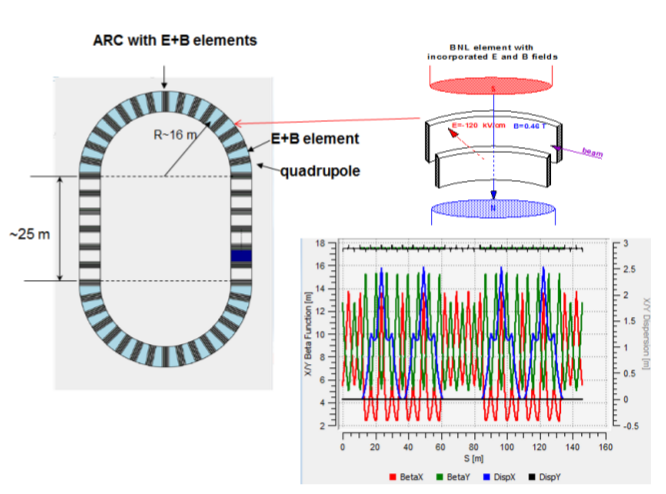
\includegraphics[width=\linewidth]{chapter2/BNL_lattice}
\end{frame}
\begin{frame}\frametitle{Симуляция}
	\begin{minipage}[t]{.48\linewidth}
		\textbf{Неидеальности\\ машины}
		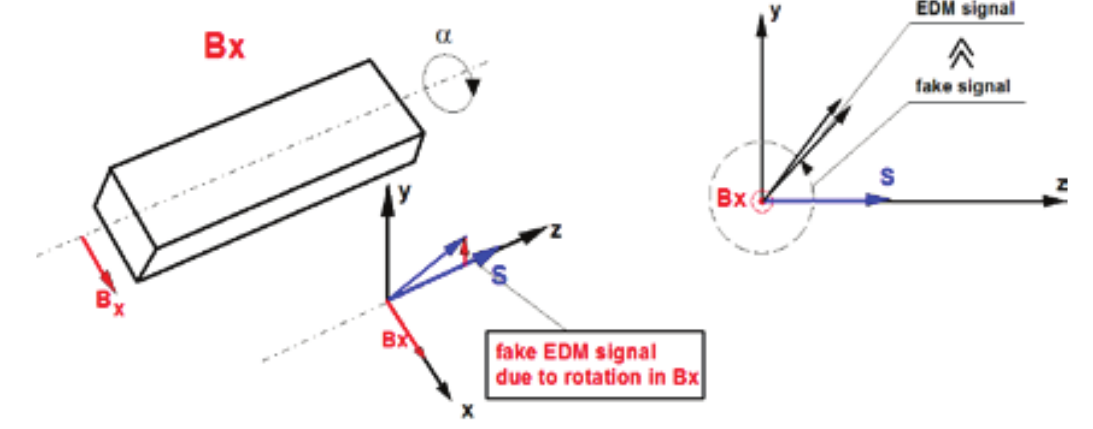
\includegraphics[width=1.2\linewidth, trim=80 10 0 0, clip]{images/magnet_tilting}
		\begin{itemize}
			\item $\alpha\sim N(\mu_i, 3\cdot10^{-4})^\circ$
			\item $\mu_i$ симулирует Спин-Колесо 
		\end{itemize}
	\end{minipage}~~~~
	\begin{minipage}[t]{.45\linewidth}
		\textbf{Частицы}
		\begin{itemize}
			\item бетатронные колебания в вертикальной плоскости
			\item $E_{FS}\neq E_{kin}\to E_{FS}$
			\item[$\Rightarrow$] $\nbar_x\ll 1 \Rightarrow$ повышенная чувствительность к возмущениям
		\end{itemize}
	\end{minipage}
\end{frame}
\begin{frame}\frametitle{Анализ}
	\begin{minipage}[t]{.5\linewidth}
		\textbf{Данные}
		\begin{itemize}
			\item[TRK] данные трекера TR COSY Infinity
			\item[GEN] вычислены по формуле, $\nbar$, $\nu_s$ вычислены на данном обороте
			\item[IDL] как в GEN, но $\nbar = \avg{\nbar}$, $\nu_s = \avg{\nu_s}$ 
		\end{itemize}
	\end{minipage}~~~~
	\begin{minipage}[t]{.5\linewidth}
		\textbf{Сравнительные\\ статистики}
		\begin{itemize}
			\item[$\epsilon_1(t)$] $= s_y^{gen}(t) - s_y^{idl}(t)$
			\item[$\epsilon_2(t)$] $= s_y^{trk}(t) - s_y^{idl}(t)$
		\end{itemize}
%		\textbf{Что сделал}
%		\begin{itemize}
%			\item Оценил пригодность модели при фитировании данных $s_y^{trk}$, $s_y^{gen}$, $s_y^{idl}$
%			\item Сравнил поведение стандартных отлклонений $\epsilon_1$, и $\epsilon_2$ относительно поведения $\sigma[\nbar]$
%		\end{itemize}
\end{minipage}
\end{frame}
\begin{frame}\frametitle{Результаты}
	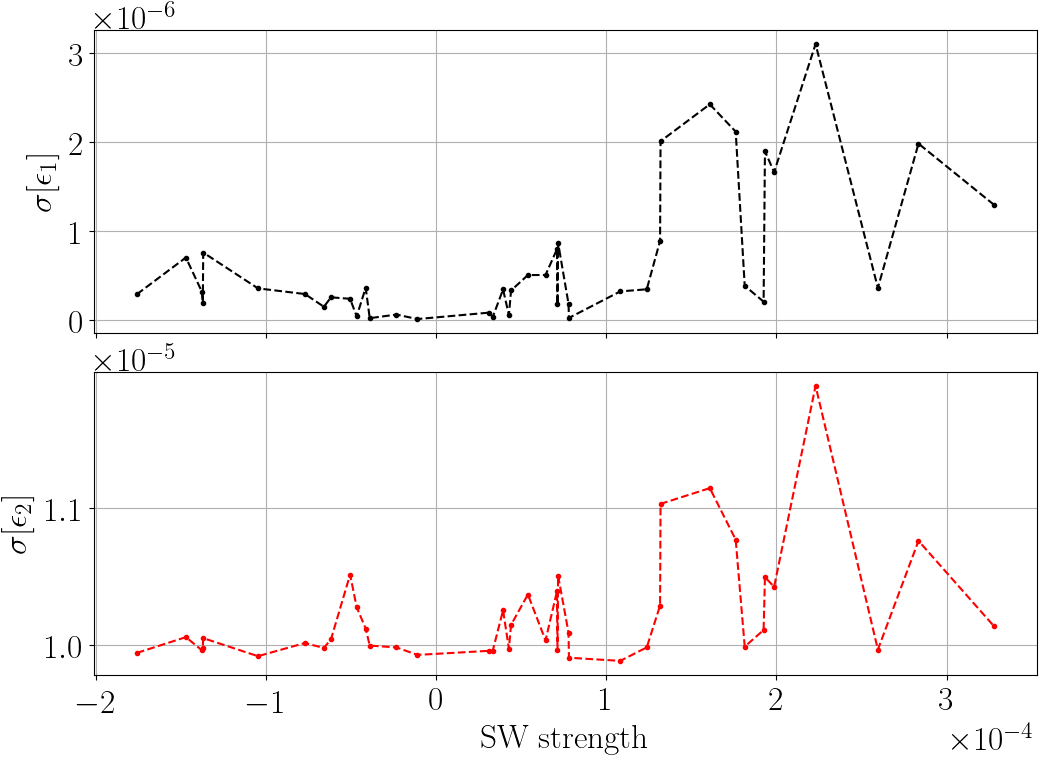
\includegraphics[width=\linewidth]{smp_sim/residual_SD_vs_SW(both)}
\end{frame}
\begin{frame}\frametitle{Результаты}
	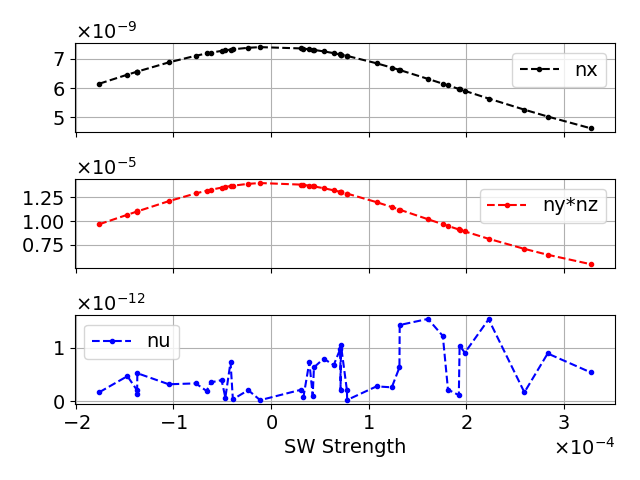
\includegraphics[width=\linewidth]{smp_sim/NBAR_variation_sd_vs_SW}
\end{frame}
\begin{frame}\frametitle{Выводы}
	\begin{enumerate}
		\item Влияние вариации $\nbar$ на дисперсию невязки между идеальными данными, и трекерными, незначительно, по сравнению с вариацией $\nu_s$
		\item $\sigma[\epsilon_2] \ll \sigma[P_y]$, значит суперпозиция систематической ошибки со случайной ошибкой измерений поляризации не будет обладать статистически значимой систематичностью
	\end{enumerate}
\end{frame}
\begin{frame}\frametitle{Выводы}
	\begin{enumerate} \setcounter{enumi}{2}
		\item $\sigma[\hat a, \hat b] < 10\%$, значит даже если вариация $\nbar$ будет достаточной, чтобы повлиять на $\hat a$, её эффект на $\hat b$ будет уменьшен как минимум в 10 раз
		\item Этот систематический эффект контролируем. Увеличивая скорость вращения Спин-Колеса, мы непрерывно уменьшали амплитуду колебаний $\nbar$
	\end{enumerate}
\end{frame}

\begin{frame}\frametitle{Декогеренция спинов}% Здесь надо добавить (более качественную) анимацию декогеренции
	\centering
	\animategraphics[autoplay,loop,height=.8\paperheight]{1}{images/spin_decoh/spin_decoh-}{0}{5}
\end{frame}
\begin{frame}{Декогеренция спинов}
	\framesubtitle{Причины}
	\begin{minipage}{.65\linewidth}
		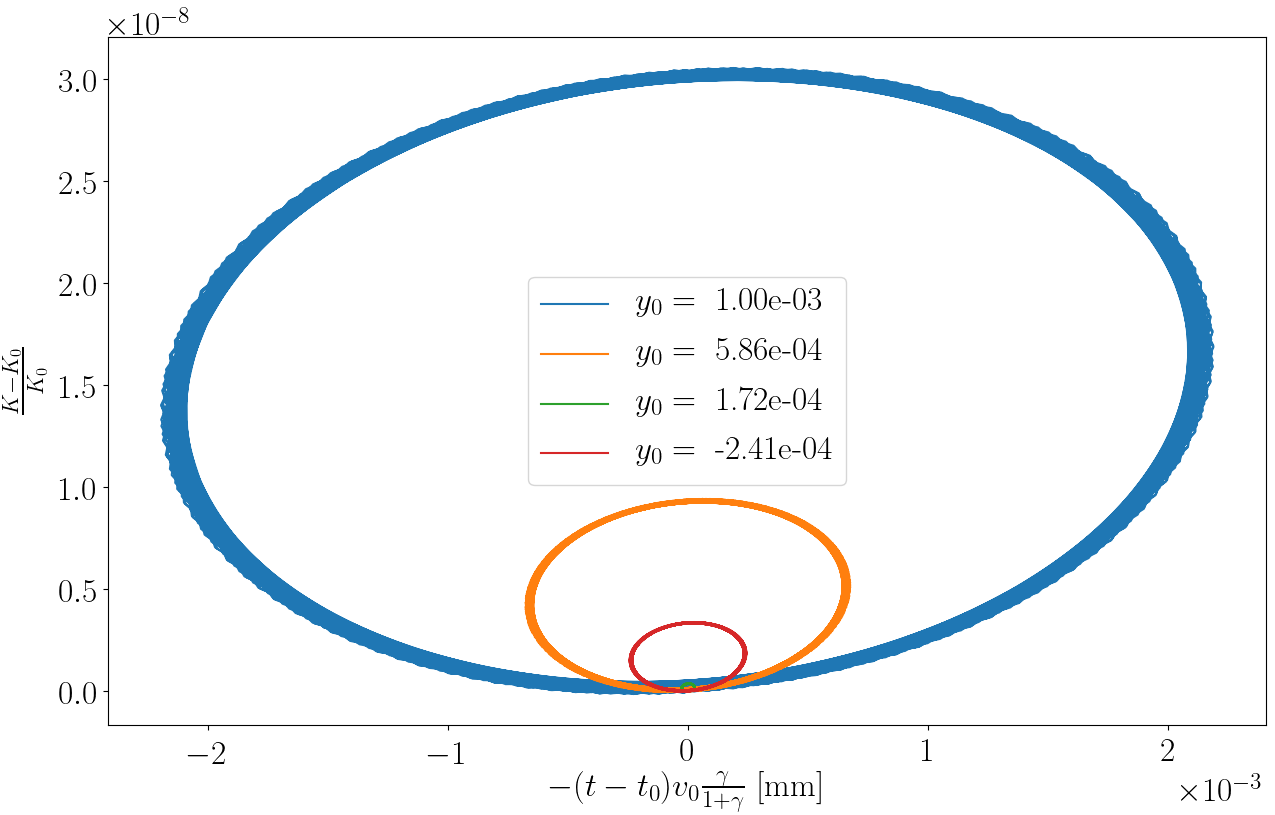
\includegraphics[width=\linewidth]{chapter1/psp_diagram_betatron}
	\end{minipage}%
	\begin{minipage}{.4\linewidth}
		\begin{itemize}
			\item $\nu_s = \gamma G$
			\item из-за разницы длин орбит, у частиц в пучке разная $\gamma_{eq}$ 
		\end{itemize}
	\end{minipage}
\end{frame}
\begin{frame}{Декогеренция спинов}
	\framesubtitle{Подавление секступольными полями}
	\begin{block}{Сдвиг равновесного уровня импульса}
		$\Delta\delta_{eq} = \frac{\gamma_0^2}{\gamma_0^2\alpha_0 - 1}\bkt*{\frac{\delta_m^2}{2}\bkt{\alpha_1 - \alpha_0\gamma^{-2} + \gamma_0^{-4}} + \bkt{\frac{\Delta L}{L}}_\beta}$
	\end{block}
	\begin{block}{Эффекты секступольных полей}
		\begin{forest}
			forked edges,
			for tree={edge={->},  rounded corners, grow'=0}
			[{$S_{sext} = \frac{1}{B\rho} \pddx{B_y}[x][2]$}
			[{$\Delta \alpha_{1,sext} = -\frac{S_{sext}D_0^3}{L}$}]
			[{$\bkt{\frac{\Delta L}{L}}_{sext} = \mp \frac{S_{sext}D_0\beta_{x,y}\varepsilon_{x,y}}{L}$}]
			]
		\end{forest}
	\end{block}
\end{frame}
\begin{frame}{Эффект секступольных полей}
	\framesubtitle{Коэффициент сжатия орбиты}
	\begin{tikzpicture}
		\node (main) {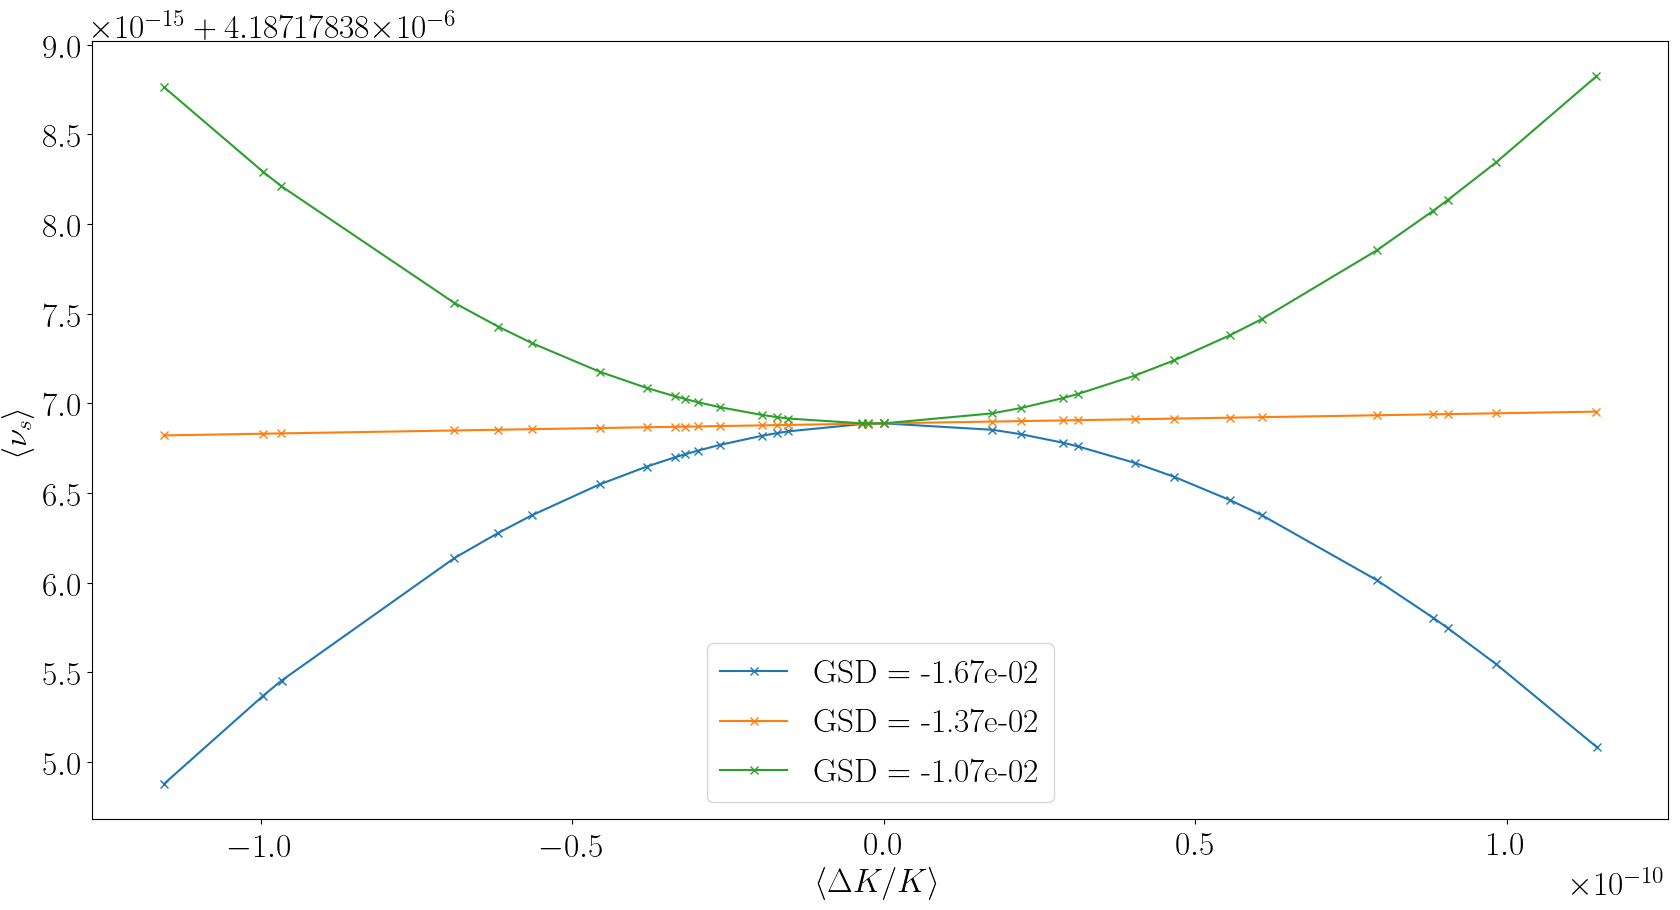
\includegraphics[width=.7\linewidth]{decoh_sim/propdef/stune_vs_dkok_SS_D}};
		\pause
		\node (PS) at (main.east)[yshift=-2cm, xshift=-.8cm] {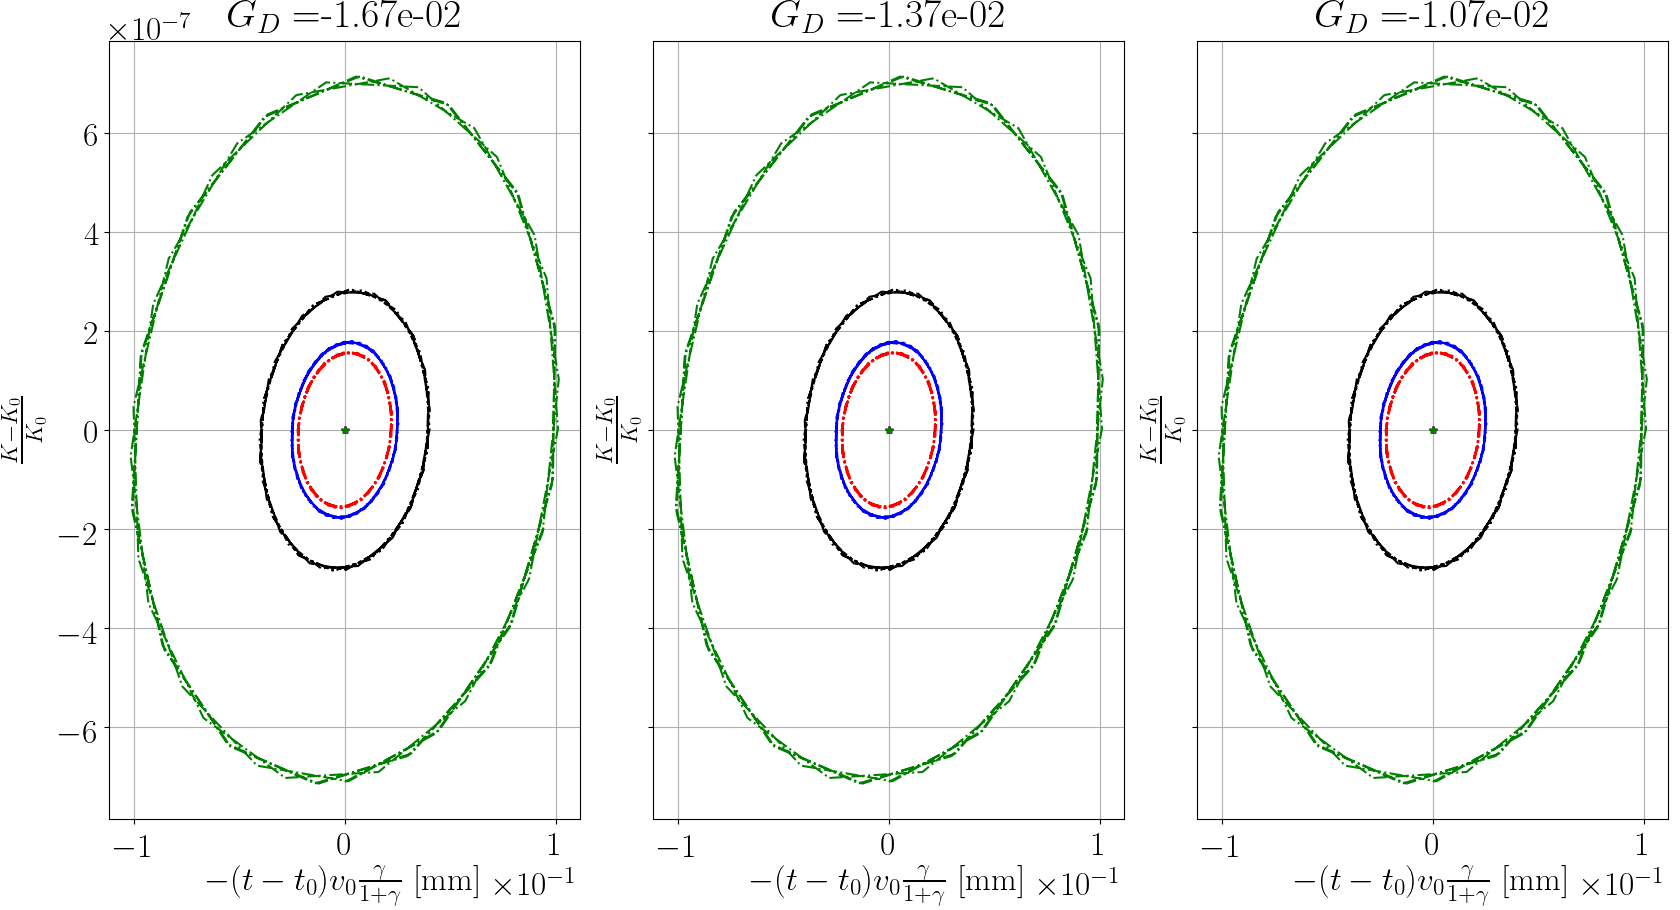
\includegraphics[width=.7\linewidth]{decoh_sim/propdef/long_phase_space_for_sext_settings_D}};
	\end{tikzpicture}
\end{frame}
\begin{frame}{Эффект секступольных полей}
	\framesubtitle{Длина орбиты}
	\begin{tikzpicture}
		\node (main) {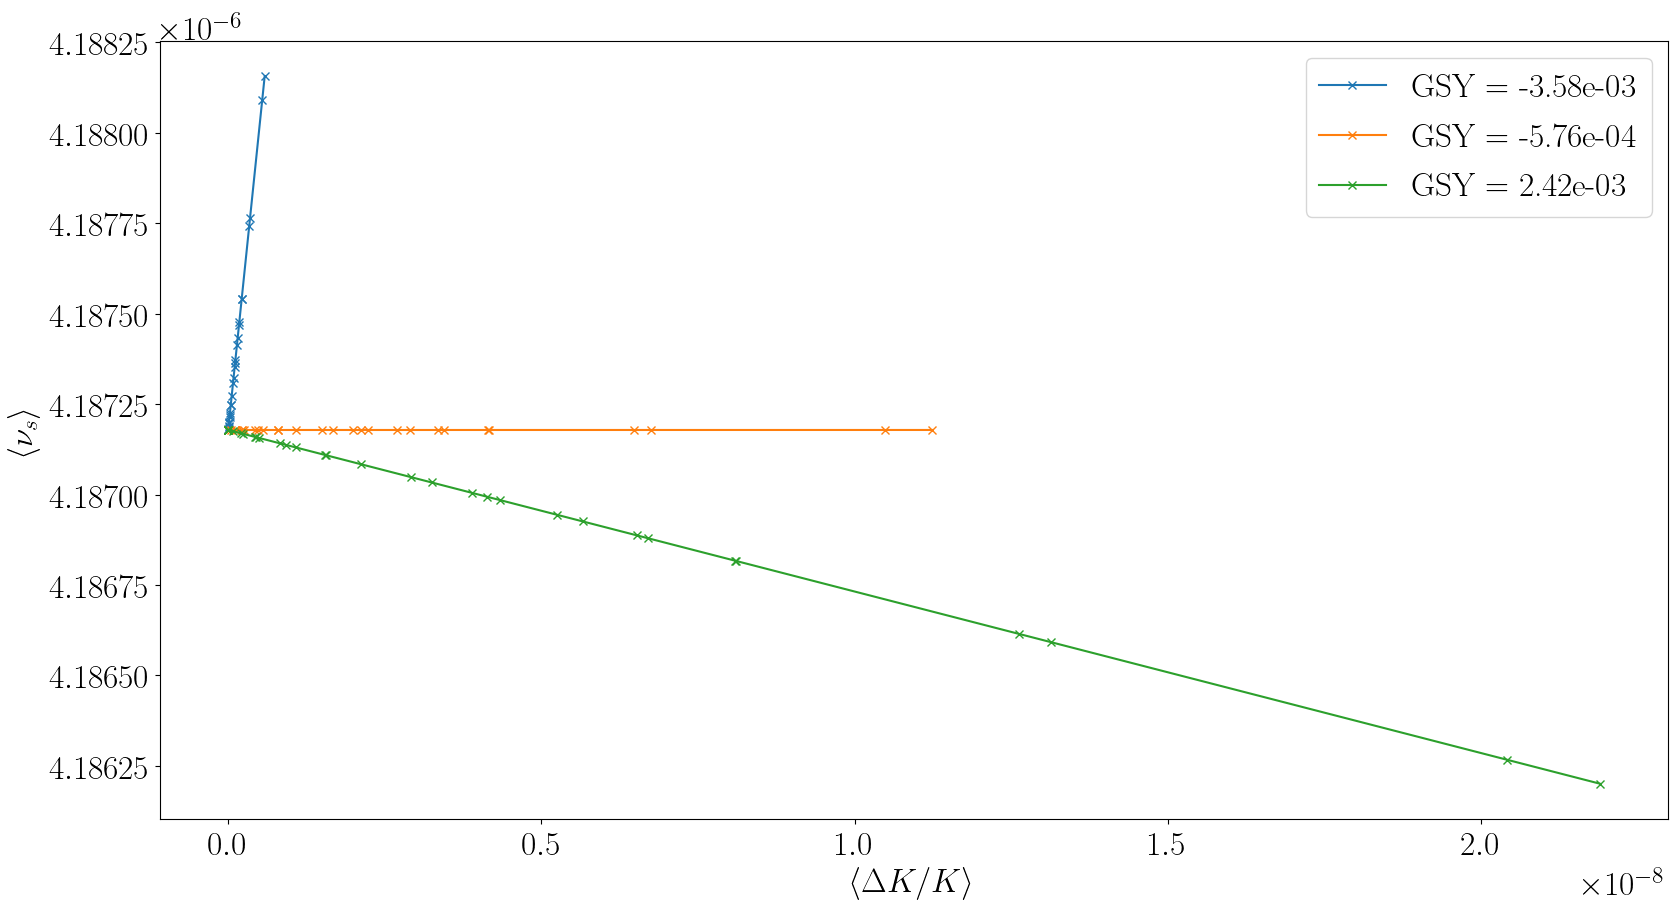
\includegraphics[width=.7\linewidth]{decoh_sim/propdef/stune_vs_dkok_SS_Y}};
		\pause
		\node (PS) at (main.east)[yshift=-2cm, xshift=-.8cm] {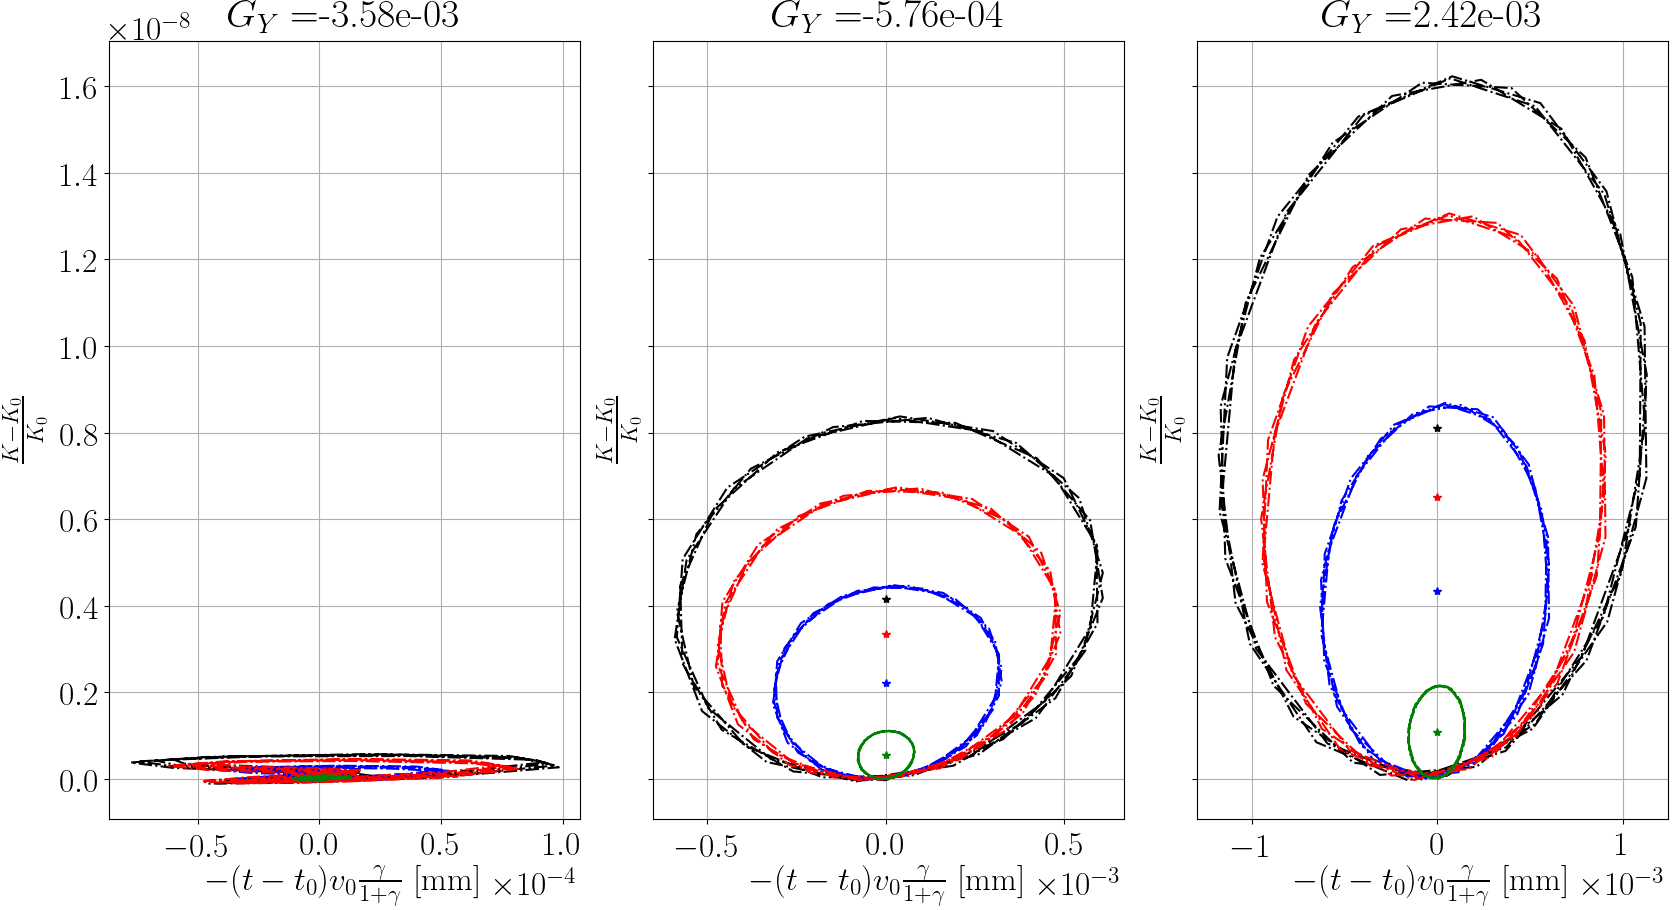
\includegraphics[width=.7\linewidth]{decoh_sim/propdef/long_phase_space_for_sext_settings_Y}};
	\end{tikzpicture}

\end{frame}
\begin{frame}{Выводы}
	\begin{enumerate}
		\item Сигнатура эффекта секступольных полей на коэффициент сжатия орбиты --- изменение функциональной зависимости $\avg{\nu_s}(\avg{\Delta K/K})$
		\item \ldots~ на длины орбит частиц банча --- уменьшение дисперсии $\avg{\Delta K/K}$
	\end{enumerate}
\end{frame}
\begin{frame}{Подавление декогеренции в идеальной структуре}\centering
	\begin{tikzpicture}
		\node (X) {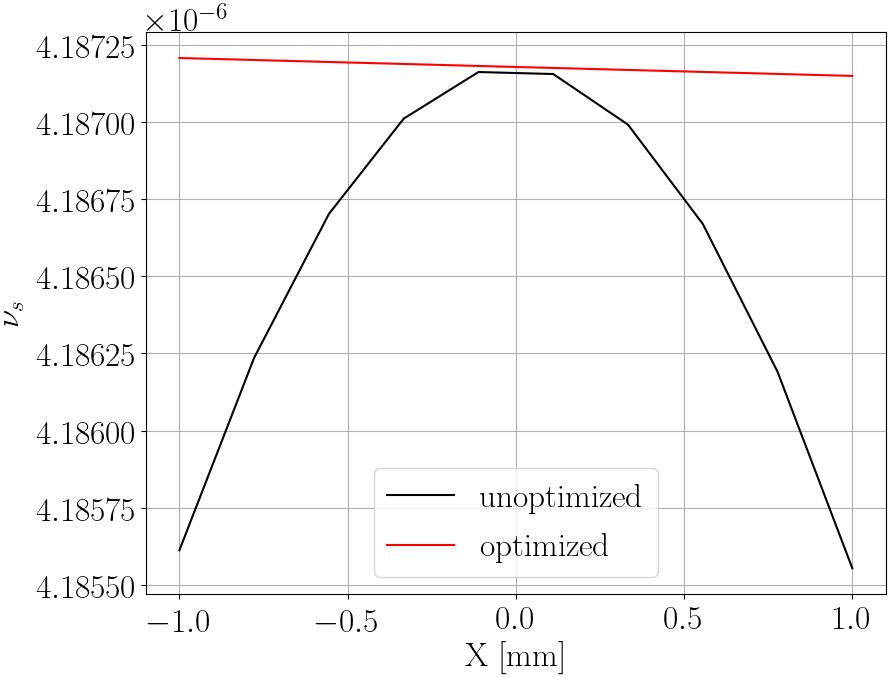
\includegraphics[height=.5\paperheight]{decoh_sim/spin_tune_decoh_x_offset}};
		\pause
		\node (Y) at (X.east)[yshift=-1.7cm]{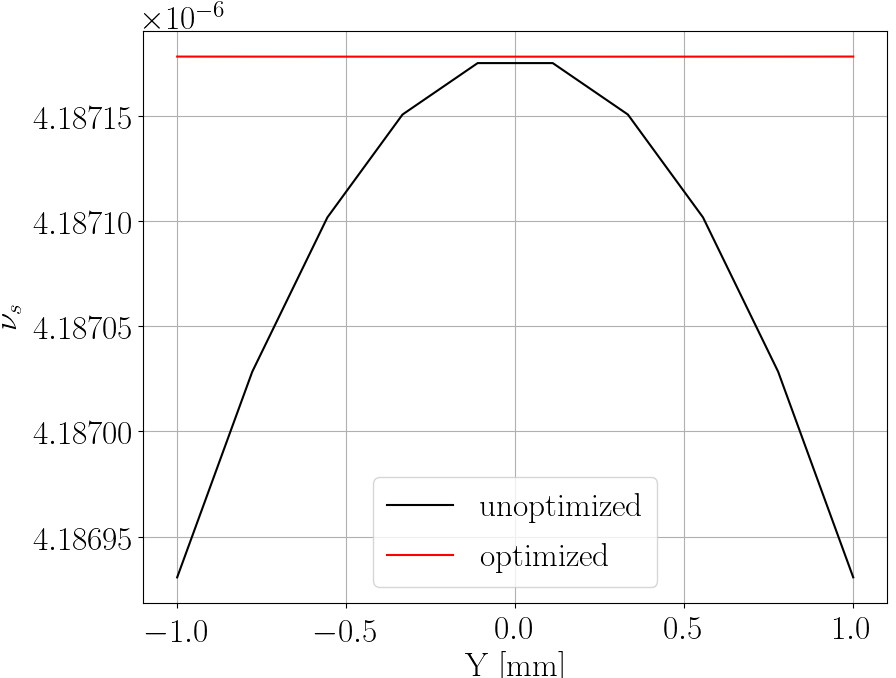
\includegraphics[height=.5\paperheight]{decoh_sim/spin_tune_decoh_y_offset}};
		\pause
		\node (D) at (X.center)[yshift=-2.3cm]{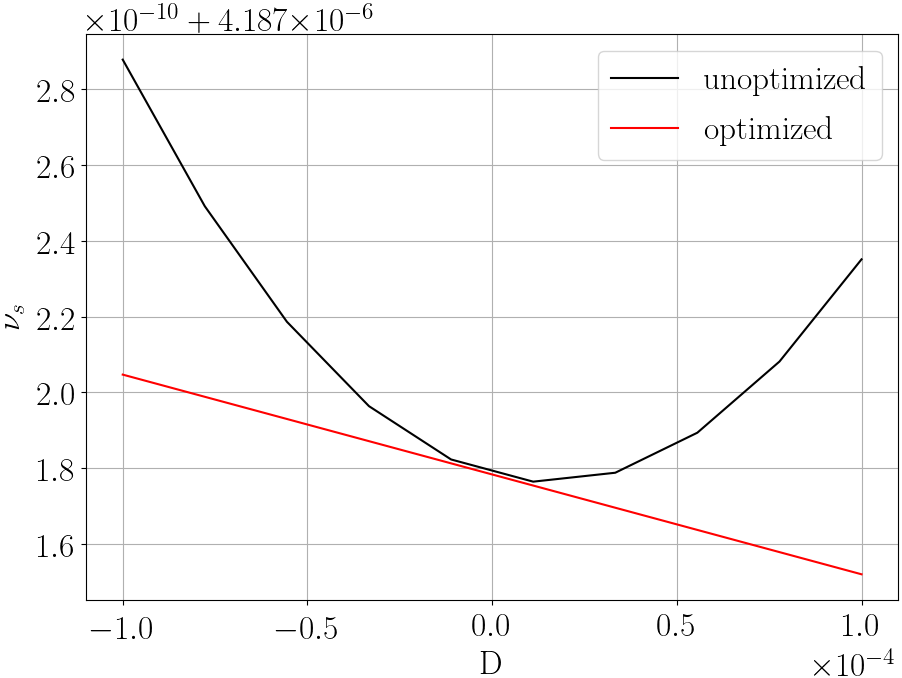
\includegraphics[height=.5\paperheight]{decoh_sim/spin_tune_decoh_d_offset}};
	\end{tikzpicture}
\end{frame}
\begin{frame}{Декогеренция в неидеальной структуре}
	\begin{tikzpicture}
		\node (imgX) {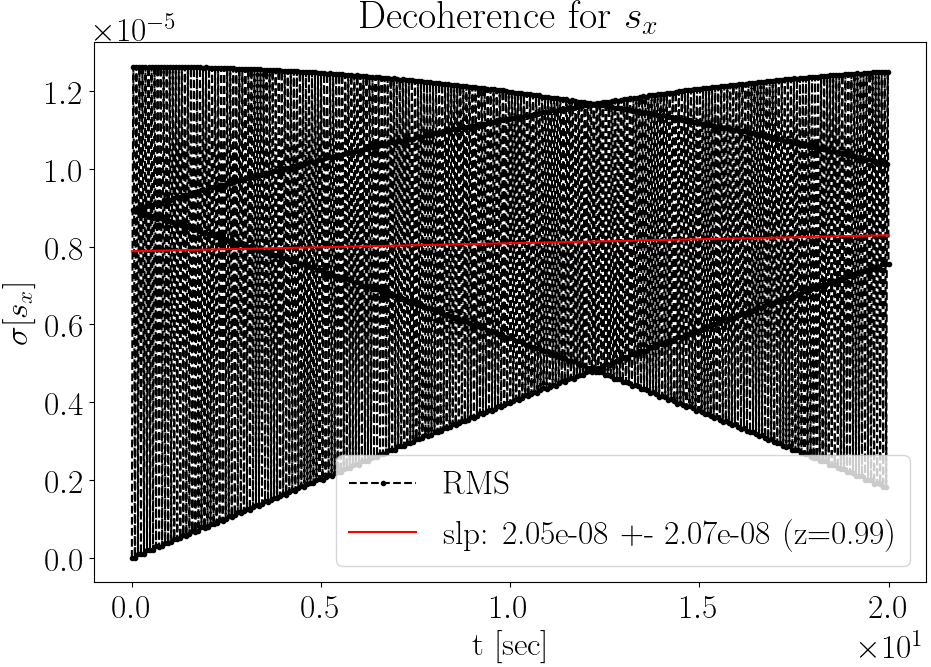
\includegraphics[width=.65\linewidth]{decoh_sim/SX_decoh_20sec_unopt}};
		\pause
		\node (imgY) at (imgX.south east)[yshift=1cm]{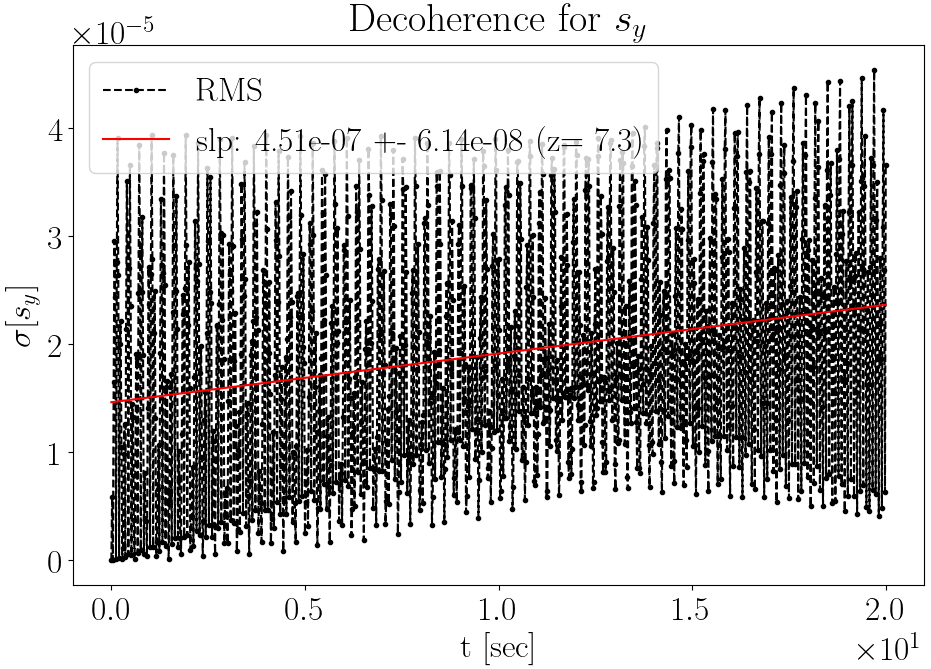
\includegraphics[width=.65\linewidth]{decoh_sim/SY_decoh_20sec_unopt}};
	\end{tikzpicture}
\end{frame}
\begin{frame}{Включаем секступоли}
\begin{tikzpicture}
\node (imgX) {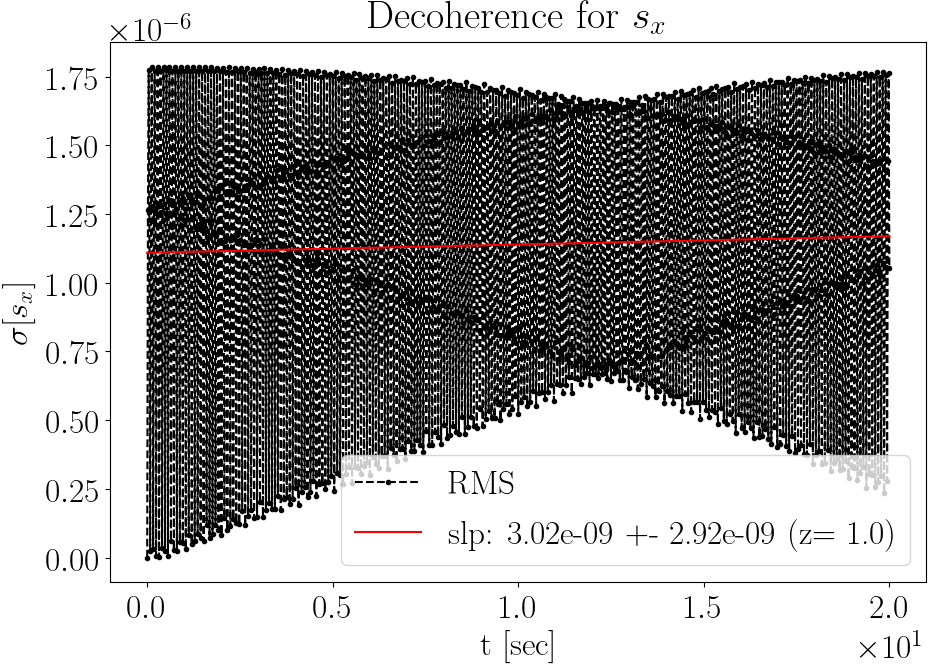
\includegraphics[width=.65\linewidth]{decoh_sim/SX_decoh_20sec_opt}};
\pause
\node (imgY) at (imgX.south east)[yshift=1cm]{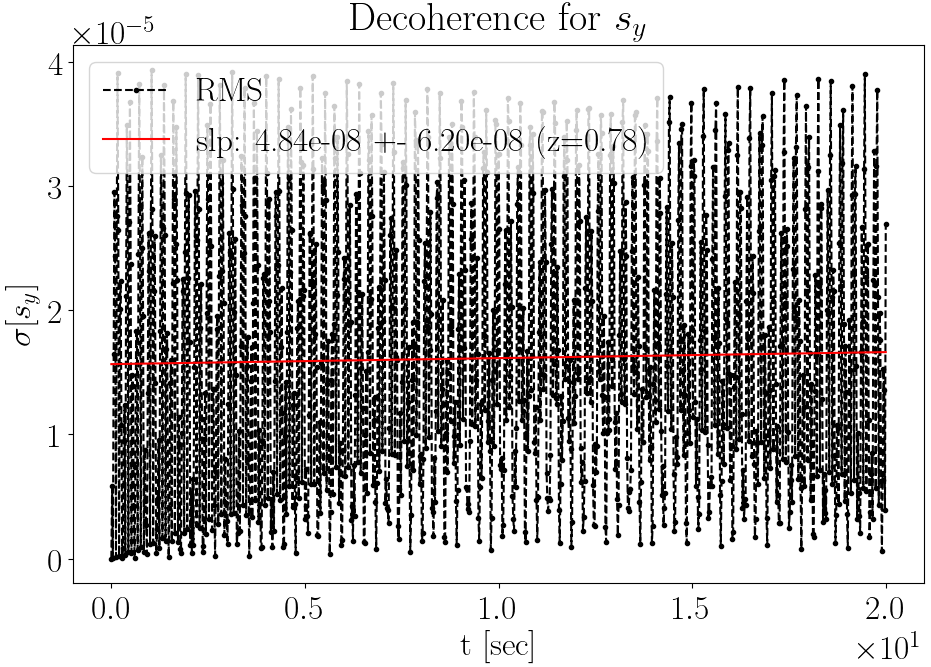
\includegraphics[width=.65\linewidth]{decoh_sim/SY_decoh_20sec_opt}};
\end{tikzpicture}
\end{frame}
%%%%%%%%%%%%%%%%%%%%%%%%%%%%%%
\begin{frame}
\frametitle{Перспективы развития проекта}
\begin{itemize}
  \item Поляризованная программа на ускорительном комплексе НИКА, ОИЯИ, Дубна
\end{itemize}
\end{frame}

\begin{frame}
\frametitle{Результаты работы}
\begin{itemize}
  \item Изучены эффекты спиновой динамики, составляющие систематические ошибки эксперимента:
  \begin{itemize}
  	\item возмущения спиновой динамики, вызванные бетатронным движением
  	\item декогеренция спинов
  	\item МДМ прецессия, связанная с неидеальностью машины
  \end{itemize}
  \item Описаны средства борьбы с каждым из эффектов, проведено численное моделирование
\end{itemize}
\end{frame}
\begin{frame}
	\begin{itemize}
		  \item Сформулированы понятия:
		\begin{itemize}
			\item методов пространственной и частотной областей
			\item двумерно-замороженного спина
			\item необходимые условия успешного измерения ЭДМ в накопительном кольце
			\item методология, удовлетворяющая этим условиям
		\end{itemize}
		\item Описаны структуры с замороженным и квази-замороженным спином
	\end{itemize}
\end{frame}

\begin{frame}
\begin{center}
Спасибо за внимание!
\end{center}
\end{frame}

\end{document} 
